\section{General concept}\label{sec:general-concept}
"Flutter is an app SDK for building high-performance, high-fidelity apps for iOS, Android, web (beta), and desktop (technical preview) from a single codebase."\cite{flutterTechnicalOverview}
It means you need only one development team to reach an application for all platforms in a single codebase.

"The goal is to enable developers to deliver high-performance apps that feel natural on different platforms.
We embrace differences in scrolling behaviors, typography, icons, and more."\cite{flutterTechnicalOverview}

Thanks to this, we can style our application user interface on demand, and the application looks similar to both platforms.

\begin{figure}
    \centering
    \begin{minipage}{.45\textwidth}
        \centering
        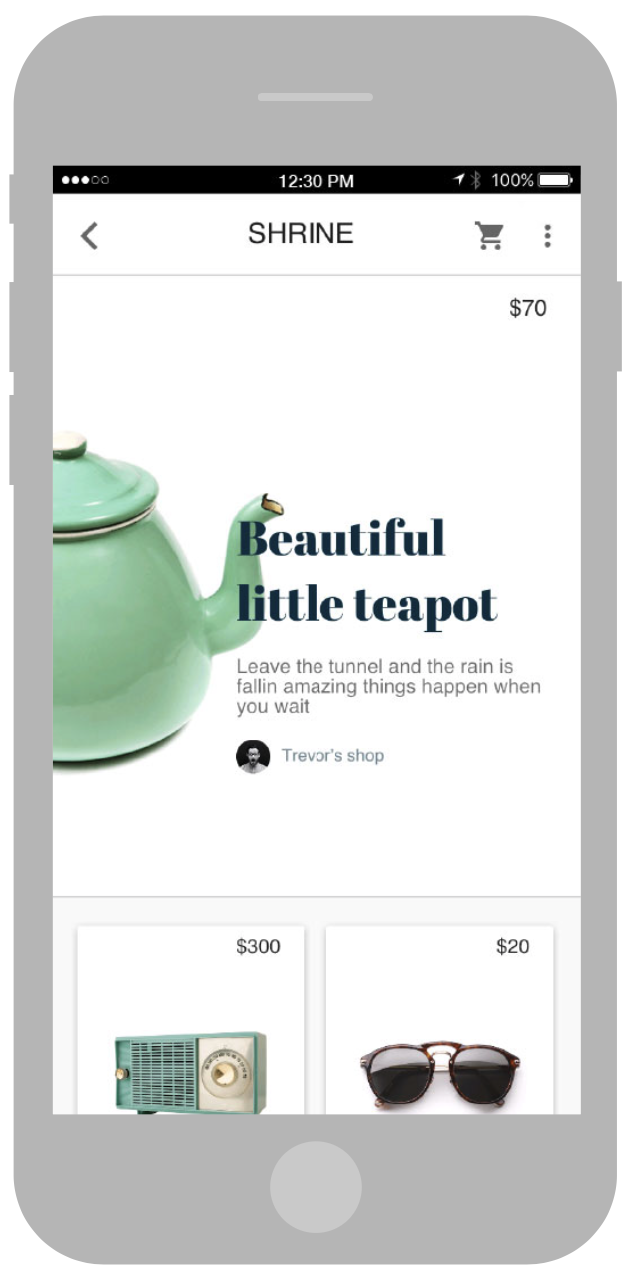
\includegraphics[width=.7\linewidth]{assets/hero-shrine-ios.png}
        \caption{Flutter demo app on iOS \cite{flutterTechnicalOverview}}
        \label{fig:flutter-demo-app-ios}
    \end{minipage}%
    \hspace{.05\linewidth}
    \begin{minipage}{.45\textwidth}
        \centering
        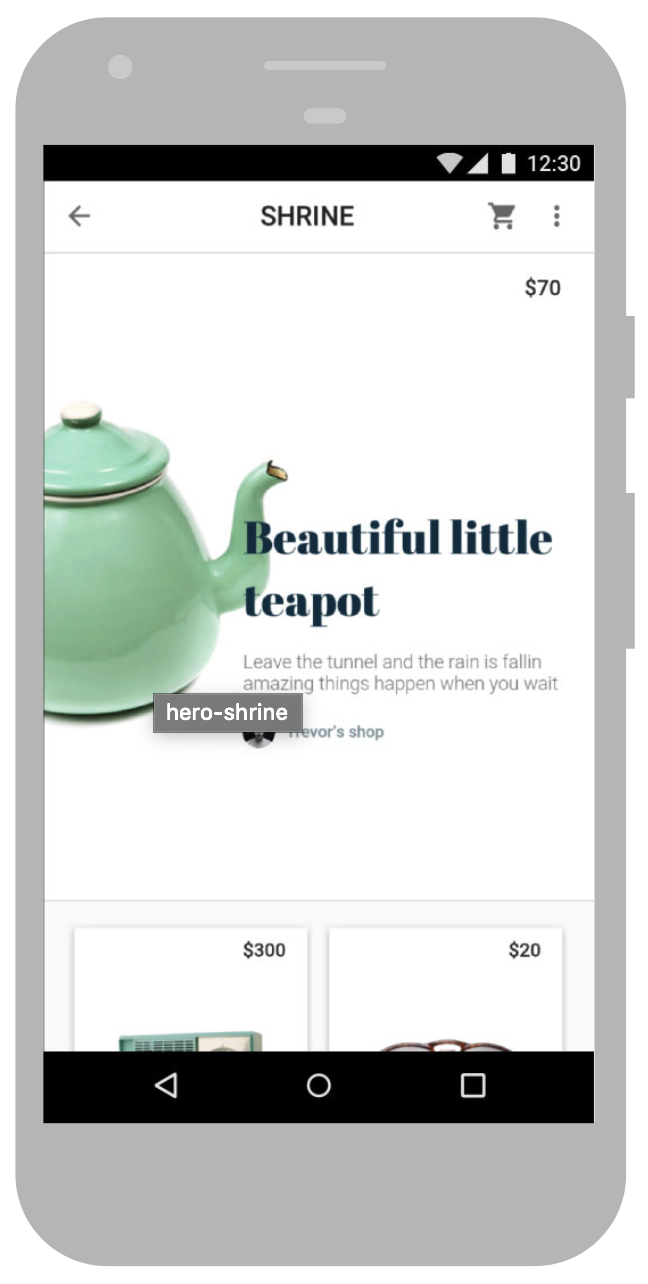
\includegraphics[width=.7\linewidth]{assets/hero-shrine-android.png}
        \caption{Flutter demo app on Android \cite{flutterTechnicalOverview}}
        \label{fig:flutter-demo-app-android}
    \end{minipage}
    \label{fig:flutter-demo-app}
\end{figure}